\documentclass[11pt]{scrartcl}
\usepackage[sexy]{evan}

\newcommand{\St}{\mathrm{St}}
\newcommand{\M}{\mathcal{M}}
\newcommand{\R}{\mathbb{R}}
\newcommand{\grad}{\operatorname{grad}}
\newcommand{\sym}{\operatorname{sym}}
\newcommand{\tr}{\operatorname{tr}}

\begin{document}
\title{AM 220 HW 3}
\author{Haozhe (Stephen) Yang}
\date{\today}
\maketitle

\section{Problem 1}

\begin{enumerate}[(a)]
    \item Note that we have the objective function is \[f(X) = \frac 12 \sum b_{ij} (x_{ij} - \tilde m_{ij})^2\]
    So we see that the derivative wrt $x_{ij}$, which is $b_{ij}(x_{ij} - \tilde m_{ij})$. Thus, putting every entry together, we see that the gradient is \[\nabla_X f = (X - \tilde M) \odot B\]
    \item Here we will use the chain rule. We see that in Fréchet's notation, we have \begin{align*}
    D_{R,L}g\bigl[\Delta R,\Delta L\bigr]
    &=\bigl\langle\nabla_x f,\;D_R X[\Delta R]\bigr\rangle
    +\bigl\langle\nabla_x f,\;D_L X[\Delta L]\bigr\rangle,\\
    D_R X[\Delta R]&=L\bigl(\Delta R\bigr)^{\top} \implies \bigl\langle\nabla_x f,\;L(\Delta R)^{T}\bigr\rangle
    =\bigl\langle(\nabla_x f)^{T}L,\;\Delta R\bigr\rangle \\
    D_L X[\Delta L]&=\Delta L\,R^{\top} \implies \bigl\langle\nabla_x f,\;\Delta L\,R^{T}\bigr\rangle
    =\bigl\langle(\nabla_x f)\,R,\;\Delta L\bigr\rangle
    \end{align*}
    Thus, it follows that \begin{align*}
        \nabla_L f &= \left[(LR^\top-\tilde M)\odot B \right] \cdot R \\
        \nabla_R f &= \left[(LR^\top - \tilde M) \odot B\right]^\top \cdot L
    \end{align*}
    \item Note that the gradient is additive, so we just find the gradient of the last term and add it to the precious answer. We can use the same method as before, write $Y = L^\top L - R^\top R$ and $h = \norm{Y}_F^2$. So we have that \begin{align*}
    D_{L,R}h\bigl[\Delta L,\Delta R\bigr]
    &=2\,\bigl\langle Y,\;D_{L}Y[\Delta L]\;-\;D_{R}Y[\Delta R]\bigr\rangle,\\
    D_{L}Y[\Delta L]
    &=\Delta L^{\top}L + L^{\top}\Delta L \\ 
    D_{R}Y[\Delta R]
    &=\Delta R^{\top}R + R^{\top}\Delta R \\
    D_{L,R}h\bigl[\Delta L,\Delta R\bigr]
    &=2\,\Bigl\langle Y,\;\Delta L^{\top}L + L^{\top}\Delta L
    \;-\;\bigl(\Delta R^{\top}R + R^{\top}\Delta R\bigr)\Bigr\rangle.
    \end{align*}
    Rewriting each inner product via 
    \(\langle A,B\rangle=\langle A^{\top},B^{\top}\rangle\) gives
    \[
    D_{L,R}h\bigl[\Delta L,\Delta R\bigr]
    =\bigl\langle 4\,L\,Y,\;\Delta L\bigr\rangle
    +\bigl\langle -4\,R\,Y,\;\Delta R\bigr\rangle.
    \]
    So putting it all together, we see that \begin{align*}
        \nabla_L g_\mu &= \left[(LR^\top - \tilde M) \odot B \right] \cdot R + \mu L \cdot \left[L^\top L - R^\top R\right] \\
        \nabla_R g_\mu &= \left[(LR^\top - \tilde M) \odot B\right]^\top \cdot L - \mu R \cdot \left[L^\top L - R^\top R\right]
    \end{align*}
    \item Let $(L,R)\in\mathcal{M}_1$ with $\operatorname{rank}(L)=\operatorname{rank}(R)=r$. We first compute the QR decompositions: $L = Q_L R_L$ and $R = Q_R R_R$. We see that $(L')^\top L' = (R')^\top R'$ iff \[J^\top R_L^\top R_L J = J^{-1}R_R^\top R_R J^{-\top}\]
    by expanding the terms (and the orthogonal $Q$ will cancel out). Thus, write $\mathcal L = R_L^\top R_L$, $\mathcal R = R_R^\top R_R$ and $\mathcal J = JJ^\top$. We see that the above equation is asking us to find a matrix $\mathcal J$ such that \[\mathcal J \mathcal L = \mathcal R \mathcal J^{-1}\]
    In particular, let $A = \mathcal L^{1/2} \mathcal R \mathcal L^{1/2}$. We can take $\mathcal J = \mathcal L^{-1/2}A^{1/2}\mathcal L^{-1/2}$. So we see that \[\mathcal {JLJ} = \mathcal L^{-1/2} A^{1/2} A^{1/2}\mathcal L^{-1/2} = \mathcal R \implies \mathcal J \mathcal L = \mathcal R \mathcal J^{-1}\]
    So we see that by taking this choice of $\mathcal J$ satisfies the desired condition. So we can just this choice of $\mathcal J$ to recover the underlying $J$.

    This consequently implies that We can turn the regularization term to 0. This means that for any $L$ and $R$ that minimizes the objective function, we can take such $J$ as found, and transform $L$ and $R$. Hence, we see that the optimum $X$ has a choice of $L$ and $R$ that guarentees the regularization term to be zero. Thus, the additional term does not alter the set of optimal $X^*$, it only helps keep the column norms of $L$ and $R$ balanced, improving numerical stability.
\end{enumerate}

\newpage

\section{Problem 2}

\begin{enumerate}[(a)]
    \item Since \(\M_2 = \St(m,r)\times\R^{n\times r}\),  
    \[
    T_{(X,Y)}\M_2
      = T_X\St(m,r)\;\times\;\R^{n\times r},
    \]
    and differentiating with respect to the contraint gives the equation of the tangent space. So take the derivative of \(X^{\top}X=I_r\) shows
    \[
    T_X\St(m,r)
      = \bigl\{Z\in\R^{m\times r}: X^{\top}Z + Z^{\top}X = 0 \bigr\}.
    \]
    Hence
    \[
    T_{(X,Y)}\M_2
      = \bigl\{(Z,W)\!: X^{\top}Z + Z^{\top}X = 0,\; W\in\R^{n\times r}\bigr\}.
    \]
    \item Write \((Z,W)\in T_{(X,Y)}\M_2\). We simply compute the retraction for each component.  
    \begin{itemize}
        \item \emph{Stiefel factor:} As given by the hint, we take $R_X(Z) = Q$ where $QR=X+Z$ is the QR-decomposition. Note that when we write $M = X+Z$, then we can take $R = (M^\top M)^{1/2}$, since $M^\top M$ is a symmetric positive definite matrix, which has a Cholesky's decomposition. Thus, we see that $Q = M (M^\top M)^{-1/2}$. In particular, \[Q^\top Q = [(M^\top M)^{-1/2} M^\top][M (M^\top M)^{-1/2}] = I_r\]
        So this choice indeed gives a valid QR-decomposition. Finally, we see that \[R_X(Z) = Q = (X+Z)((X+Z)^\top(X+Z))^{-1/2}\]
        When expanding the second term, we see that it is $X^\top X + X^\top Z + Z^\top X + Z^\top Z$. We know that $X^\top X = I_r$ and $ X^\top Z + Z^\top X = 0$ from the previous part, so the retraction simplifies to \[R_X(Z) = (X+Z)(I_r + Z^\top Z)^{-1/2}\]
        We show that this is a retraction. For $c(t) \coloneq R_X(tZ)$, $c(0) = X$, write $M(t)=I_r + t^2 Z^\top Z$. We have \begin{align*}
            \frac{d}{dt}\bigl[M(t)^{-\tfrac12}\bigr]
            &=-\tfrac12\,M(t)^{-\tfrac12}\,(2t\,Z^\top Z)\,M(t)^{-\tfrac12} \\
            &=-t\,M(t)^{-\tfrac12}(Z^\top Z)\,M(t)^{-\tfrac12},\\
            c'(t)
            &=Z\,M(t)^{-\tfrac12}
            +(X + tZ)\,\frac{d}{dt}\bigl[M(t)^{-\tfrac12}\bigr]\\
            &=Z\,(I_r + t^2 Z^\top Z)^{-\tfrac12}
            -t\,(X + tZ)\,(I_r + t^2 Z^\top Z)^{-\tfrac32}\,Z^\top Z.
        \end{align*}
        So we have $c'(0) = Z$, which shows that this is a retraction.
      \item \emph{Linear factor:} The tangent space is inside the manifold, so \(R_Y(W)=Y+W\). We can easily see that for this satisfies the definition of retraction from the linear sum.
    \end{itemize}
    Thus, \[R_{(X,Y)}(Z,W) = \bigl((X+Z)(I + Z^\top Z)^{-1/2},\,Y+W\bigr).\]
    This is a retraction from the tangent space back onto the manifold.
    \item Note that because $\mathcal M_2$ is embedded in a Euclidean space, and a natural inner product inherited from the Frobenius metric on \(\R^{m\times r}\times\R^{n\times r}\) is given by \[\left\langle (Z_1,W_1),(Z_2,W_2)\right\rangle _{(X,Y)}= \tr(Z_1^{\top}Z_2) + \tr(W_1^{\top}W_2).\]
    So we can use the metric \[d_{\mathcal M_2}((Z_1,W_1),(Z_2,W_2)) = \sqrt{\norm{Z_1-Z_2}_F^2 - \norm{W_1-W_2}_F^2}\]
    \item Let
    \[
    G \;=\;\nabla f(XY^{\!\top})
           \;=\;\bigl(XY^{\!\top}-\widetilde M\bigr)\odot B.
    \]
    By the standard chain-rule (from problem 1),
    \[
    \nabla_X^{\mathrm {euc}}g = G\,Y,
    \qquad
    \nabla_Y^{\mathrm {euc}}g = G^{\top}X.
    \]
    Now, we again consider the two components: \begin{itemize}
        \item \emph{Stiefel factor:} Project \(\nabla_X^{\mathrm {euc}}g\) onto \(T_X\St(m,r)\) via
        \(\Pi_X(A) = A - X\,\sym(X^{\top}A)\). Hence \begin{align*}
            \grad_X g &= G\,Y \;-\; X\,\sym\bigl(X^{\top}G\,Y\bigr) \\
            &= GY - \tfrac 12 X (X^\top GY + Y^\top G^\top X)
        \end{align*}
        \item \emph{Linear factor:} Note that the tangent space is the manifold, so no projection is needed, so we simply have $\grad_Y g= G^{\top}X.$
    \end{itemize}
    
    These satisfy \(\grad_X g\in T_X\St(m,r)\) and \(\grad_Y g\in\R^{n\times r}\). So this is indeed the Riemannian gradient.
\end{enumerate}

\newpage

\section{Problem 3}

\begin{enumerate}[(a)]
    \item Because $\mathcal M_3$ is embedded in $\RR^{m\times n}$, then we see that the tangent space is also in $\RR^{m\times n}$, so for any two vectors on the tangent space, they are both in a linear subspace of $\RR^{m\times n}$. Hence, we can just compute their inner product by the Frobenius inner product on the greater space, so \begin{align*}
        &\bigl\langle (U',M',V'),\,(U'',M'',V'')\bigr\rangle \\
        =& \bigl\langle U M' V^{\top} + U' V^{\top} + U (V')^{\top},\,
                    U M'' V^{\top} + U'' V^{\top} + U (V'')^{\top}\bigr\rangle\\
        =& \tr\bigl(M'^{\top}M''\bigr)
        + \tr\bigl(U'^{\top}U''\bigr)
        + \tr\bigl(V'^{\top}V''\bigr).
    \end{align*}
    \item We simply want to prohect the Euclidean gradient down to the tangent space. In particular, we have that \[G=\nabla_X^{\text{euc}} f(X)\;=\;(X-\widetilde M)\odot B.\]
    So we just want $Y \in T_x(\mathcal M_3)$. Note that we can just project down to each component. For $U$ the projection is $P_U = UU^\top$, and for $V$ it is $P_V = VV^\top$. Note that we can write $G$ as \[G = P_UZ P_V + (1-P_U) Z P_V + P_UZ (1-P_V) + (1-P_U)Z (1-P_V)\]
    We see that the first term is projecting down to the $UMV^\top$ block; the second term is projecting down to the $U'V^\top$ block; the third term is projecting down to the $U(V')^\top$ block; and the last term is the orthogonal part to all the components. Therefore, we see that under the projection on to the tangent space, the gradient with respect to each component had been written out, we have \[P_U \; G + G \; P_V - P_U \; G \; P_V\]
    So if we let \[
        \begin{aligned}
        M_g &= U^{\top}\,G\,V,\\
        U_g &= \bigl(I - U U^{\top}\bigr)\,G\,V,\\
        V_g &= \bigl(I - V V^{\top}\bigr)\,G^{\top}\,U.
        \end{aligned}
    \]
    We see that the projected gradient down to each component is \[\grad f(X) = (U_g, M_g, V_g) \in T_x(\mathcal M_3)\]
    with the matrix form $\text{Proj}_{T_x(\mathcal M_3)}(G) = U_g V^{\top} + U M_g V^{\top} + U (V_g)^{\top}$.
\end{enumerate}

\newpage

\section{Problem 4}

The Jupyter Notebook can be found on my GitHub: \href{https://github.com/haozheyang42/AM220-
Homeworks/blob/main/hw3/hw3.ipynb}{https://github.com/haozheyang42/AM220-
Homeworks/blob/main/hw3/hw3.ipynb} I will also include code snippets in the pdf.

\bigskip

Across the three manifolds, the objective function is identical. The only difference is the geometry we impose on the search space. We obtain the following results on $(m, n, r) = (200, 500, 5)$: \begin{center}
    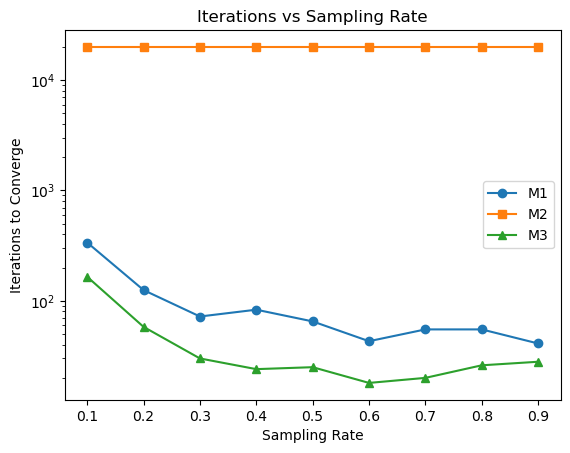
\includegraphics[width=7cm]{hw3-img/hw3-p4-1.png}
    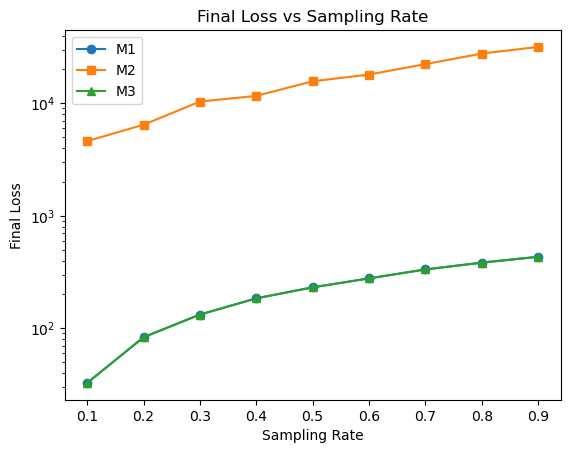
\includegraphics[width=7cm]{hw3-img/hw3-p4-2.png}
\end{center}

I set the maximum number of iterations to \(25{,}000\). The flat orange line at the top of the first plot shows that on \(\mathcal{M}_2\) the solver always runs out of iterations without ever getting \(\|\mathrm{grad}\,f\|<10^{-4}\). By contrast, both \(\mathcal{M}_1\) and \(\mathcal{M}_3\) finish in less than 100 steps. I believe this happens because: \begin{itemize}
    \item \(\mathcal{M}_1\) is just plain Euclidean space, so the optimization is smooth and fast. There are no constraints or curved directions to worry about, and each gradient step goes straight downhill. In fact, this is the same setting you see in textbook gradient descent, where the landscape is well understood and numerical solvers are highly tuned. 
    \item On \(\mathcal{M}_3\), we do even better by working directly on the set of fixed-rank matrices. We parameterize \(X=U\Sigma V^\top\), so every point we consider already has the right rank. That means there's no back-and-forth between high and low rank, and the algorithm never wastes steps correcting scale or rank errors. Each move takes us closer to the true solution with minimal detours.
    \item By contrast, \(\mathcal{M}_2\) forces one factor onto the Stiefel manifold (orthonormal columns) while leaving the other factor free. This mix creates two issues: you have to perform expensive retractions and vector transports on the Stiefel side, and you still suffer from the usual scale ambiguity on the free side. The result is a mismatched geometry where gradient directions in one factor don't line up cleanly with those in the other. The solver ends up zig-zagging and often stalls, which is why \(\mathcal{M}_2\) takes so many iterations without making real progress.
\end{itemize}

As for the loss, we see that the loss curves grow roughly linearly with the number of observed entries because each new sample adds more noise to the fit. For \(\mathcal{M}_1\) and \(\mathcal{M}_3\), the two loss curves looks identical and appears linear (even though I plotted it as log-scale but they should still be linear). This is simply because the model is not capturing the noise. Essentially, sampling more data simply uncovers more random fluctuations from the noise. By contrast, \(\mathcal{M}_2\)'s loss curve is shifted significantly higher at every sampling level. Its solver never reaches the true noise floor (after the max limit of $25,000$), so the curve stays elevated and shows irregular jumps when progress stalls. This persistent gap in loss highlights that \(\mathcal{M}_2\) fails to capture the underlying signal as accurately as the other two approaches.

Moreover, I ran simulation for $(m, n, r) = (500, 1000, 20)$, and got the following results: \begin{center}
    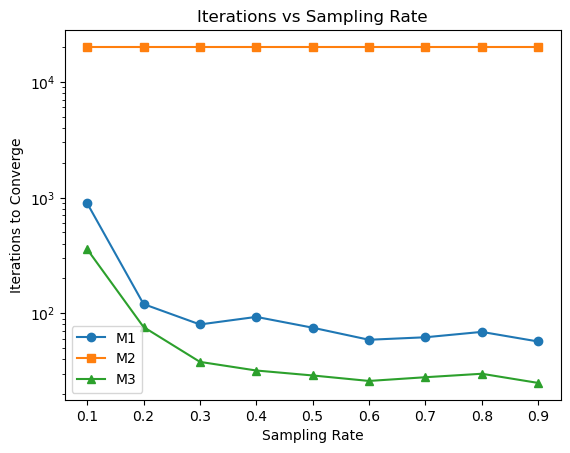
\includegraphics[width=7cm]{hw3-img/hw3-p4-3.png}
    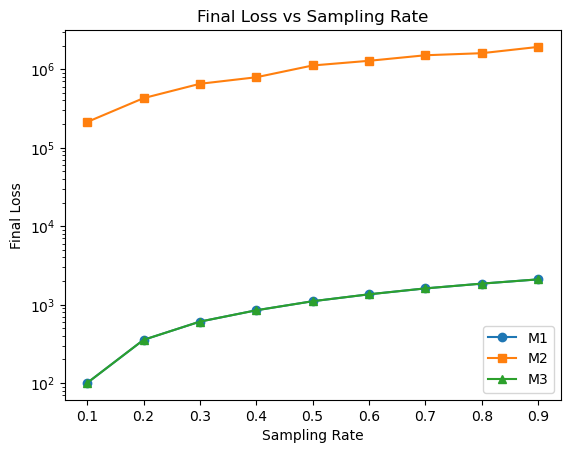
\includegraphics[width=7cm]{hw3-img/hw3-p4-4.png}
\end{center}
As we can see the iterations went up for $\mathcal M_1$ and $\mathcal M_3$. Obviously $\mathcal M_2$ is still stuck at max iterations without improvement. Moreover, we see that loss for $\mathcal M_1$ and $\mathcal M_3$ still appears linear, which represents that the underlying noise is causing the loss. This further supports what I believe as discuss previously.

Here is the implementation of the code:
\paragraph{Defining the manifold}
\begin{verbatim}
manifold1 = Product([
    Euclidean(m, r),
    Euclidean(n, r)
])
manifold2 = Product([
    Stiefel(m, r),
    Euclidean(n, r)
])
manifold3 = FixedRankEmbedded(m, n, r)
\end{verbatim}

\paragraph{Generating the test data}
\begin{verbatim}
def generate_data(m, n, r, rate):
    U_true = np.random.randn(m, r)
    V_true = np.random.randn(n, r)
    M_true = U_true @ V_true.T

    sampling_rate = rate
    B = (np.random.rand(m, n) < sampling_rate).astype(float)
    # M_tilde = M_true * B

    noise_std = 0.1
    noise = noise_std * np.random.randn(m, n)
    M_tilde = (M_true + noise) * B
    return M_tilde, B
\end{verbatim}

\paragraph{Gradient Descent}

\begin{verbatim}
# Approach 1
@pymanopt.function.autograd(manifold1)
def cost1(L, R):
    G = (anp.dot(L, R.T) - M_tilde) * B
    return 0.5 * anp.linalg.norm(G, 'fro')**2

problem1 = pymanopt.Problem(manifold=manifold1, cost=cost1)
solver1 = SteepestDescent(max_iterations=25000, min_gradient_norm=1e-4, verbosity=1)
result1 = solver1.run(problem1)

L_opt, R_opt = result1.point
X_opt1 = L_opt @ R_opt.T
E1 = (X_opt1 - M_tilde) * B
print("Approach 1 final loss:", 0.5 * np.linalg.norm(E1, 'fro')**2)

# Approach 2
@pymanopt.function.autograd(manifold2)
def cost2(X, Y):
    G = (anp.dot(X, Y.T) - M_tilde) * B
    return 0.5 * anp.linalg.norm(G, 'fro')**2

problem2 = pymanopt.Problem(manifold=manifold2, cost=cost2)
solver2 = SteepestDescent(max_iterations=25000, min_gradient_norm=1e-4, verbosity=1)
result2 = solver2.run(problem2)

X_opt, Y_opt = result2.point
X_opt2 = X_opt @ Y_opt.T
E2 = (X_opt2 - M_tilde) * B
print("Approach 2 final loss:", 0.5 * np.linalg.norm(E2, 'fro')**2)

# Approach 3
@pymanopt.function.autograd(manifold3)
def cost3(U, S, V):
    # reconstruct the rank-r matrix
    X = anp.dot(U, anp.dot(anp.diag(S), V))
    E = (X - M_tilde) * B
    return 0.5 * anp.linalg.norm(E, "fro")**2

problem3 = pymanopt.Problem(manifold=manifold3, cost=cost3)
solver3 = SteepestDescent(max_iterations=25000, min_gradient_norm=1e-4, verbosity=1)
result3 = solver3.run(problem3)

# Extract the optimal X
U_opt, S_opt, V_opt = result3.point
X_opt3 = anp.dot(U_opt, anp.dot(anp.diag(S_opt), V_opt))
E3 = (X_opt3 - M_tilde) * B
print("Approach 3 final loss:", 0.5 * np.linalg.norm(E3, "fro")**2)
\end{verbatim}

\end{document}